\chapter{System Design and Implementation}\label{chap:methods}\label{chap:impl}
We build a system that writes online (live) match updates for Age of Empires II (AoE2) using high-fidelity game data. In this chapter, we present both the system design and a prototype implementation in a system we call Semantic Abstraction \& Generation from Events (\textit{SAGE}\footnote{The inclusion of "AGE" for Age of Empires II is intentional, although we believe the high-level framework is generalizable to other domains.}). We connect our earlier analysis (desired narrative structure and how it relates to available data) to a concrete architecture and spell out the constraints for a live system (e.g., no future knowledge, low latency). We then describe how we implement this design for our evaluation, including data preparation (Section~\ref{sec:data-preparation}), pipeline stage implementations (Section~\ref{sec:pipeline-implementation}), and the architectural modules.

\section{Design Requirements}
The related work and domain analysis (Chapters~\ref{chap:background}, ~\ref{chap:prelim}, ~\ref{chap:viewer-study}) together translate into the following design requirements, which directly support the Research Goals in Chapter~\ref{chap:introduction} and guide the architecture of SAGE:

\begin{enumerate}
  \item \textbf{Narrative Coherence:} The system must move beyond a linear log of events to create a coherent story that respects the causal and temporal relationships of the match, showing how parallel events connect, while prioritizing the most critical moments.
  \item \textbf{Strategic Contextualization:} The system must use CaptureAge's deep data to generate insights that would typically require a human expert, such as identifying a strategy or a critical mistake.
  \item \textbf{Linguistic Alignment:} The system must use linguistic techniques identified in professional shoutcasting (such as specific information and vocabulary) to produce text that informs and engages.
\end{enumerate}

\section{Pipeline Design}
SAGE follows the modular pipeline architecture established by \citet{reiter2000} and exemplified by BabyTalk \cite{reiter2007}: Signal Analysis $\rightarrow$ Data Interpretation $\rightarrow$ Document Planning $\rightarrow$ Microplanning and Realization. This framing provides explicit control over content selection and cleanly supports the ablation design required by our evaluation. In practice our approach is hybrid: the first three stages perform rule-based content selection, while Realization uses an LLM-based Realizer (Section~\ref{sec:pipeline-implementation}).

Classic pipelines such as BabyTalk \cite{reiter2007} operate over continuous numeric signals, with Signal Analysis separating numeric from symbolic inputs. Our inputs differ: a symbolic event stream and periodic game-state snapshots rather than continuous signals. Moreover the developments of the past few years towards Large Language Models (LLMs) have changed the way the realisation steps are performed.

\subsection{Operational Constraints}
There are specific constraints for our live data-to-text setting that shape the design of each stage and the overall architecture:

\begin{itemize}
  \item \textbf{Live operation:} data arrives incrementally; the system must plan and realize text without knowledge of future events.
  \item \textbf{Low latency:} minimal gaps between events and reporting \cite{lewandowski2012} require incremental upstream processing and a Realizer optimized for low first-token latency.
  \item \textbf{Textual-only medium:} without shared visuals, commentary compensates with explicit spatial anchoring, temporal framing, and named actors.
  \item \textbf{Modularity:} enrichment and structuring behaviors must be independently switchable (enabling or disabling each separately) to empirically test whether the design requirements improve viewer engagement. Concretely, Narrative Coherence and Strategic Contextualization are each operationalized as optional architectural modules (\textit{Event Structuring} and \textit{Expert Insights} respectively; Section~\ref{sec:modules}). This enables an ablation study downstream to measure their effect on engagement metrics.
\end{itemize}

Across stages, a database provides event and state information as well as numerical constants and metadata. We refer to the first three stages collectively as \textit{Content Selection} and the last as \textit{Realization}. The following subsections describe our inputs and target output, our event model for content selection, and finally how the pipeline stages are specialized for our setting.

\subsection{Inputs and Target Output}
\subsubsection*{Inputs}
Our pipeline receives two kinds of live input: a symbolic event stream and game state snapshots. While this is not a stream of continuous numeric signals like BabyTalk, the event stream still requires analysis (e.g., clustering), and the snapshots provide the context needed for interpretation.
\begin{itemize}
  \item \textbf{Event stream}: typed events, for example damage dealt, unit trained, technology status changed. \footnote{Command events (all player inputs) also exist, but we do not use them downstream in this project due to data corruption issues in the source recording files. This is a limitation, but it also helps us focus solely on game-state-driven events.}
  \item \textbf{Game state snapshots}: positions, actions, visibility, projectiles, populations, resources for each unit and player at specific points in time.
\end{itemize}
Here, with "stream" we mean that data arrives incrementally such that it can be operated on incrementally, supporting live operation. Snapshot data is a copy of the game state at a specific point in time. For a fuller description of the raw inputs, see Appendix~\ref{appendix:data-schema}. Section~\ref{sec:data-preparation} provides practical details on how we process these inputs.

\subsubsection*{Target Output Structure}
Based on the domain analysis findings in Chapter~\ref{chap:prelim}, we want the pipeline output content to be structured as follows:
\begin{itemize}
  \item Create an introductory segment that sets the scene for the match.
  \item Follow an event-driven loop structure, where each notable event is reported in a coherent and engaging manner.
  \item Focus on supportive state information only when it adds context to notable events, no separate state updates when there are no notable events.
  \item Omit lull-based updates to concentrate on summarization and the event-driven loop.
  \item End with a short closing segment that clearly indicates the winner and the events that led to the conclusion.
\end{itemize}

In addition to the loop and state-enhanced notable events, we need to account for the lack of a visual modality. To compensate, we add clear references to locations and when it happened, and describe the actors involved and their actions.

The output should also be engaging. We therefore follow the live text commentary and shoutcasting language findings reviewed in Chapter~\ref{chap:background} \cite{lewandowski2012,pavzanin2022,byro2017,gustin2020}. In practice, this means favoring present-tense narration, explicit temporal/spatial anchoring, and selective evaluative phrasing to convey momentum without inventing facts.

\subsubsection*{Example Target Output}

For the content selection pipeline stages, the target output structure above translates into following the cue-based Actuator--Environment--Performance+Sensors (A--E--P+S) structure identified in the domain analysis. To illustrate the accumulation of information content available to the system at each stage, we present an example of progressive enrichment for a single event. Underlined text indicates newly added or modified information at each operation.

\begin{itemize}
  \item \textbf{Base Text (Actuator/Cue):} Red's three scouts find a Villager.
  \item \textbf{E-P+S Enrichment:} \underline{With Forging now in} (\textit{Environment}), Red's three scouts find a Villager. \underline{Red is now three Villagers ahead} (\textit{Performance}).
  \item \textbf{Spatial and Temporal Language:} \underline{16:32 -- } With Forging now in, Red's three scouts find a Villager \underline{on the forward woodline}. Red is now three Villagers ahead.
  \item \textbf{Style (final):} 16:32 -- With Forging now in, Red's three scouts \underline{waste no time -- they spot} on the forward woodline! Red \underline{surges ahead with a three-Villager advantage,} \underline{and momentum is clearly shifting.}
\end{itemize}

\subsection{Pipeline Specialization}
Classic data-to-text pipelines typically operate over structured numeric records, where content selection in Document Planning chooses what to report \cite{gkatzia2016}. Our setting slightly diverges from this classical approach in two ways: inputs are symbolic game events rather than numeric signals, and periodically evolving game-state snapshots are accessed to enrich signals with contextual information. For our implementation we follow a rule-based approach informed by our preliminary analysis and a A-E-P+S-based schema: detect and cluster notable events (Signal Analysis), enrich them with snapshot context (Data Interpretation), then prioritize and structure them into a streaming narrative (Document Planning), which is then realized using LLM-based Realization.

In practice this follows four steps: (1) detect and cluster notable events, (2) enrich them with A-E-P+S context from snapshots, (3) plan a streaming narrative, and (4) realize each content unit into text.

\subsection{Event Types}
Unlike classic pipeline settings with continuous signals, our inputs are symbolic events. Game-engine events are instantaneous, but the phenomena we want to report (e.g., battles) typically span time; we therefore distinguish:
\begin{itemize}
  \item \textbf{Instant Event}: a discrete occurrence with no meaningful duration (e.g., a command, damage tick, projectile impact).
  \item \textbf{Interval Event}: an occurrence spanning a time window (e.g., a skirmish, raid, construction, relic sequence).
\end{itemize}

We also distinguish event sources:
\begin{itemize}
  \item \textbf{Base Event}: an Instant directly observed from game data (at minimum: timestamp and type).
  \item \textbf{Derived Event}: a higher-level construct formed by aggregating/translating events or snapshots (e.g., a battle interval; inferred strategies).
  \item \textbf{Synthetic Event}: system-added events used for structure (e.g., Minute-Ticks for temporal grounding).
    %   \item \textbf{Actuator Event}: an event resulting from a player's action or effect visibly changing the game world state (e.g., training a unit, constructing a building, researching a technology, or engaging in combat). These are the primary drivers of the narrative loop.
\end{itemize}

\subsection{Event Abstraction}
A core challenge is turning many low-level Instants into reportable Interval Events. Work on abstracting sequential low-level event logs into higher-level activities (e.g., process mining) provides useful framing \cite{zelst2021}, but our primary targets (battles) are not simple linear processes and cannot be represented by single instants (e.g., one unit death), we don't know if a single event will lead to a "battle", and we don't know when the "battle" ends. We therefore start with clustering of damage-related Instants into derived battle intervals, which provides the minimum abstraction needed for downstream planning and realization.

\subsection{Pipeline Stages}
The symbolic nature of our inputs and the availability of game-state snapshots require specializing two of the four pipeline stages. Signal Analysis shifts from separating and processing numeric signals to clustering and filtering symbolic Instants into higher-level Interval Events (e.g., grouping damage ticks into a battle). Data Interpretation shifts from signal-level enrichment to snapshot-based contextual enrichment, retrieving game-state information at the time of each event to support strategic explanation.

To address the "generation gap" (early commitments that later processing would revise) \cite{gatt2018}, we allow limited feedback and feedforward between stages. For example, the Document Planner may request additional contextual information (e.g., ongoing battle details) from the Data Interpreter to better handle concurrent events.
We next describe the prototype end-to-end, including data preparation (Section~\ref{sec:data-preparation}) and concrete stage implementations (Section~\ref{sec:pipeline-implementation}). Architectural modules used for ablation are described in Section~\ref{sec:modules}.

\section{Prototype Overview}
We implement the design described above as a prototype system (\textit{SAGE}). We first present a high-level view of the end-to-end data flow (Figure~\ref{fig:pipeline-base}), then detail data preparation (Section~\ref{sec:data-preparation}) and pipeline implementation (Section~\ref{sec:pipeline-implementation}).

\subsection*{Data Flows}
The data flows through the system as follows:
\begin{figure}[htbp]
  \centering
  % Avoid build errors if file is missing
  \IfFileExists{assets/pipeline-base.pdf}{%
    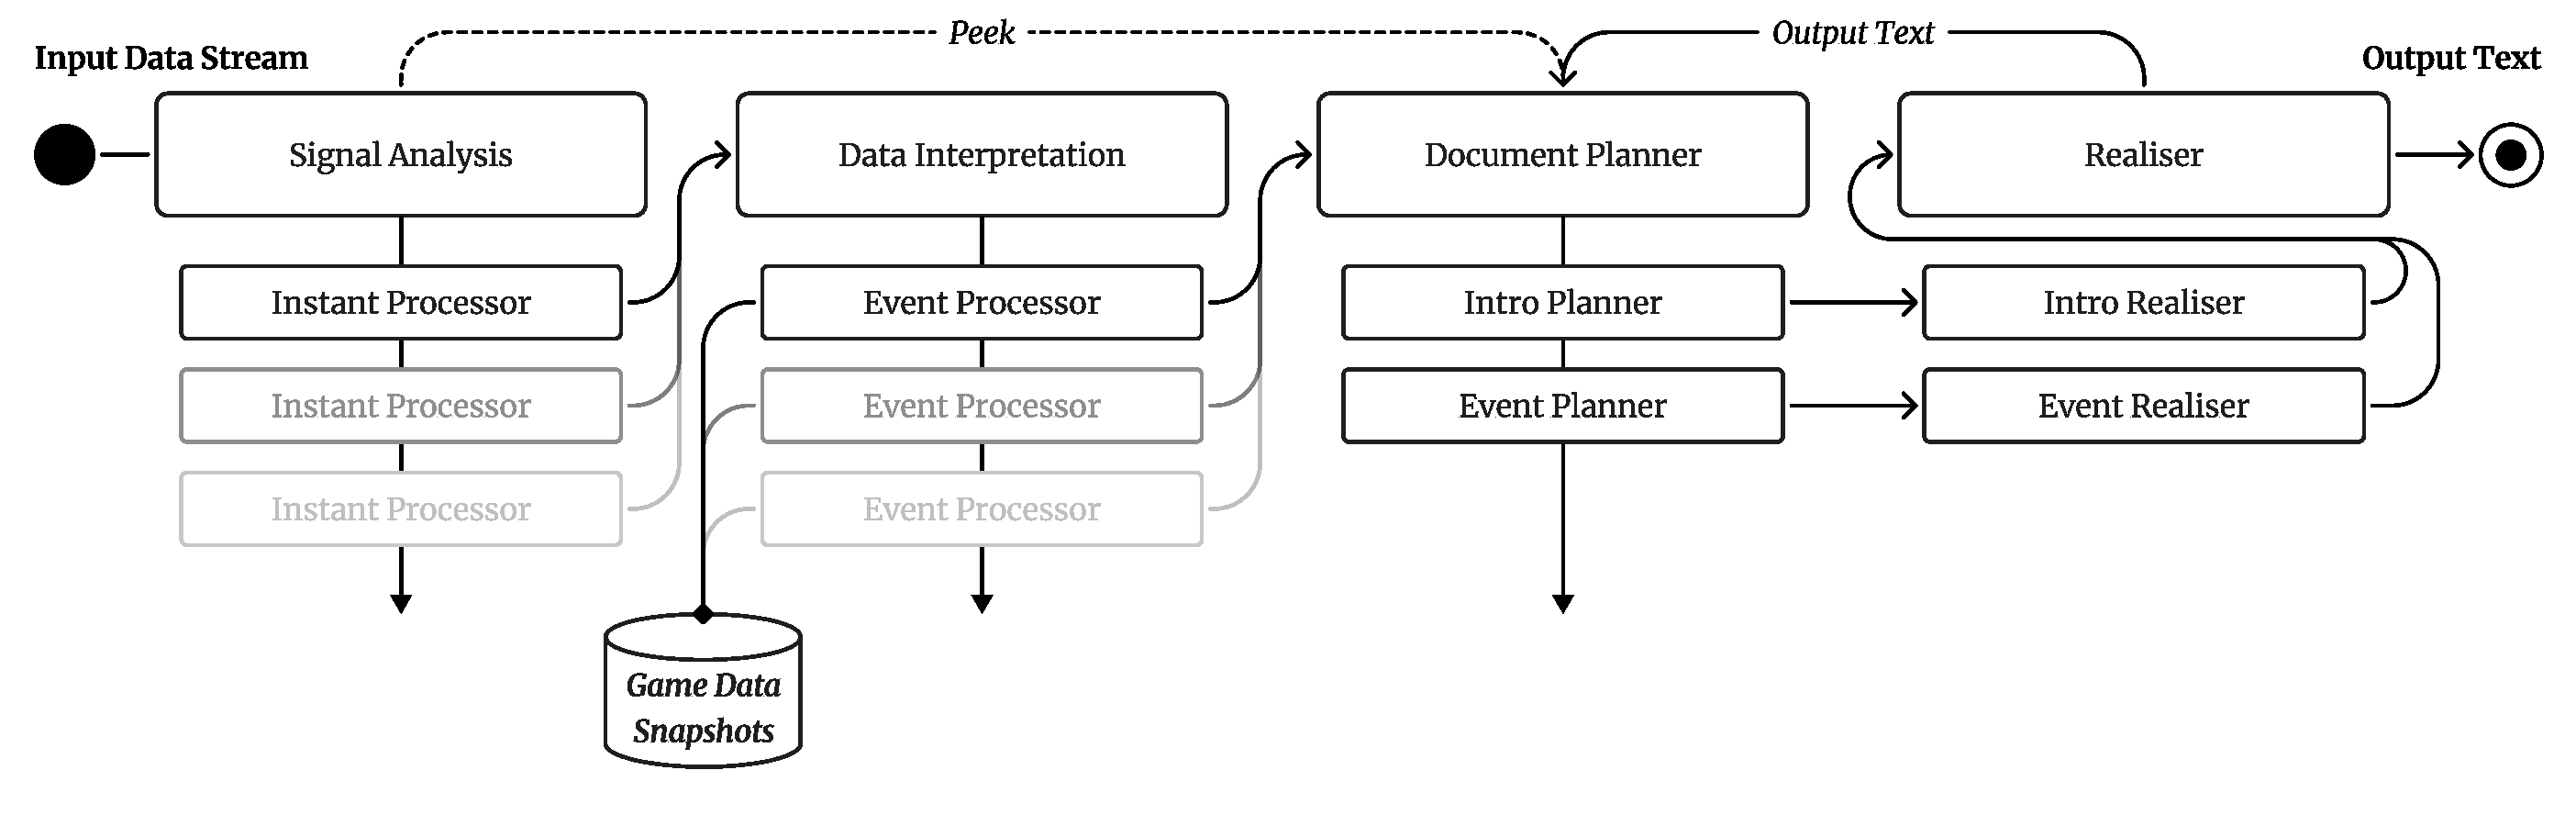
\includegraphics[width=\textwidth]{assets/pipeline-base.pdf}%
  }{%
    \fbox{\parbox{0.95\textwidth}{\centering Placeholder: missing file\\`assets/pipeline-base.pdf`}}%
  }
  \caption{High-level data flow of the \textit{SAGE} pipeline, enhanced with Age of Empires II-specific content selection and realization steps.} 
  \label{fig:pipeline-base}
\end{figure}
\begin{enumerate}
  \item Raw event data is ingested from the exported CaptureAge data in the Apache Arrow format.
  \item Events are processed through the Signal Analyzer, where they are filtered and clustered. Effectively events can be buffered until clusters are decided to be complete.
  \item Events are passed to the Data Interpreter for enrichment with contextual data from the corresponding game state snapshots.
  \item The Document Planner organizes enriched events into content units for realization. For this it can buffer events or peek at ongoing events to decide when to emit content units.
  \item Each content unit is realized into text by the LLM-based Realizer. The output is sent back to the Document Planner to allow it to provide future LLM calls with previously generated context. \footnote{Strictly speaking, we don't need to send it back, and keep it in the Realizer module, but since Document Planning and realization operate in pairs we prefer making the Realizer stateless.}
  \item Realized text segments are concatenated to form the final live text commentary.
\end{enumerate}

\section{Data Preparation}\label{sec:data-preparation}
\subsection{Recorded Games}
We retrieved recorded games with permission from King of the Desert IV\footnote{Permission kindly given by MembTV with assistance from DonDinardoni, who labeled each recorded game file for the set, players, and match numbers.}, the next installment of the tournament used in the preliminary study (Chapter~\ref{chap:viewer-study}), a year later. Recorded games--containing all player commands and starting state--were replayed in the version compatible \footnote{We used a community tool for that: \url{https://github.com/gregstein/DE-Replays-Manager/}} Age of Empires II: Definitive Edition client using an automated script via the in-game API to produce the CaptureAge data format.

\subsection{CaptureAge Data}
We extracted a subset of the recorded game data into the CaptureAge format, focusing on key events and player actions (Instants) and minute-long snapshots (60-second windows were found to have an acceptable file-size/retrieval-duration trade-off). Since Signal Analysis can buffer event data before context enrichment, the prototype needs access to previous game states to enrich events correctly. We therefore keep snapshot data as windowed state slices with incremental window identifiers (IDs) available for retrieval during interpretation; moving this state-tracking fully into ingestion may be preferable, at the cost of separation of concerns to be able to directly enrich during and avoid using out-dated state or caching large amounts of data. This also limits time-travel during enrichment: if interpretation happens later than event detection (due to buffering), we can still enrich using the snapshot that was current at the event time rather than whatever the latest state happens to be at interpretation time. However the 60-second window size may still introduce aliasing, where there never was a world state that exactly matches the event time. The dataset includes:
\begin{itemize}
  \item \textbf{Snapshot data:} Entities (units, buildings, resources), Masters (static data), Research States, Player States, and World data (time, prices).
  \item \textbf{Starting states:} Map terrain and settings (e.g., map name and dimensions; in our KotD IV dataset: Arabia, 120$\times$120 tiles).
  \item \textbf{Instants:} Entity events (e.g., created, died) and technology events.
  \item \textbf{Strings:} ID-to-text mapping.
\end{itemize}

The game lobby settings used for our recorded games are listed in Appendix~\ref{appendix:lobby-settings}. Selected snapshot data entries were annotated with metadata such as lifecycle changes (Created, Updated, Deleted, Transient --- came into and outof existence in the same window) and visibility timestamps to support debugging and event reporting. Each file is exported in the portable Apache Arrow format using Arquero \cite{arquero}, allowing for platform-agnostic efficient columnar storage and retrieval. All data is described in a descriptor schema containing the recorded game name, a list of files generated (one per type), and each file's window size and time boundaries, so window IDs can be mapped to game time\footnote{Game time is typically 1.69 times faster than real time.}. A full overview of the extracted data, including the schema and field definitions, can be found in Appendix~\ref{appendix:data-schema}.

\subsection{Dataset Scope and Release}
The evaluation corpus consists of 173 matches from King of the Desert IV, a top-level AoE2 tournament. Alongside it, we release a substantially larger dataset of 3,100 competitive matches, collected from competitive ranked 1v1 ladder matches in May 2026. Both datasets are exported at 1-second and 60-second snapshot resolutions. The full breadth of covered data types (including entities, player states, research states, command streams, world state, and significant derived events) is documented on the dataset page (Appendix~\ref{app:corpus}). To our knowledge, no comparable dataset exists at this level of continuous full-state telemetry for any esports title; prior work relies on sparse event logs or video feeds that do not expose structured game state directly.

\subsection{Iteration}
When iterating on the prototype, we focused on a specific configuration of the pipeline's rule-based stages (including event clustering thresholds, content prioritization rules, and narrative structure) to ensure we produced output suitable for evaluation. The following sections present the final results after this iteration. We occasionally mention other approaches we tested as well. The criteria used to assess progress and the outcomes are discussed in Section~\ref{sec:system-design-conclusion}.

Iteration is done on a single recorded game to allow for quick testing and validation. For this we chose a randomly selected game from our dataset, with a duration of approximately 45 in-game minutes, which is representative of typical match lengths. For this we picked match Group B - Round 1, Game 2 between Mbl and Vinchester from the King of the Desert IV tournament. This match features a balanced mix of battles, economy management, and strategic plays, making it suitable for testing the various modules and pipeline stages.

% \subsection{Iteration Outcomes}
% Above we described the implementation as it stands now. During the iteration process several changes were made to the design in order to reach the desired output quality and stability. Below we list some of the more significant changes:

% \begin{itemize}
%   \item We tried several different data structures and snapshot intervals. The data as described in Appendix~\ref{appendix:data-schema} contains unused data points that were retained to support iteration and potential future experiments.
%   \item We tested several different prompting techniques for the LLM-based Realizer (e.g., prompt variations, structures, few-shot vs. no-shot, alternative style descriptions) before settling on the current configuration.
%   \item We implemented and compared different detection strategies for battles and building events, as part of the original design, and pruned those that did not contribute clearly to summary quality.
%   \item We implemented an initial rule-based realization system for locations. This may be of interest as a cheap pre-realization step to support LLMs that work better with human-readable, linear text representations \cite{wang2024} instead of nested JSON structures.
%   \item We added additional data points to obtain the correct information as we developed the system (e.g., gameStatus was initially believed to contain resigned status to help indicate match endings, but this was not the case).
% \end{itemize}

\section{Pipeline Implementation}\label{sec:pipeline-implementation}
\subsection{Implementation Notes}
The prototype system for \textit{SAGE} is implemented in TypeScript, aligning with the CaptureAge tooling and allowing us to reuse existing data-processing utilities. Strong static typing helped us ensure that data is passed correctly between stages and modules, and helped highlight malformed or missing information early during development. To support this, we created a set of specialized generic types to ensure correct inference of the event types at each stage of the pipeline.
As such, the stack uses Node 22 with Yarn 4 and TypeScript 5.8. Overall, the stack is reasonably light: Arquero for reading and querying Apache Arrow, Zod for external data validation, and Remeda for functional programming utilities. We employ Jest as an iterative development aid for interactively running and debugging targeted code.

A full high-level visualization of the pipeline implementation can be found in Figure~\ref{fig:data-pipeline}.

\begin{figure}[htbp]
  \centering
  % Avoid build errors if file is missing
  \IfFileExists{assets/data-pipeline.pdf}{%
    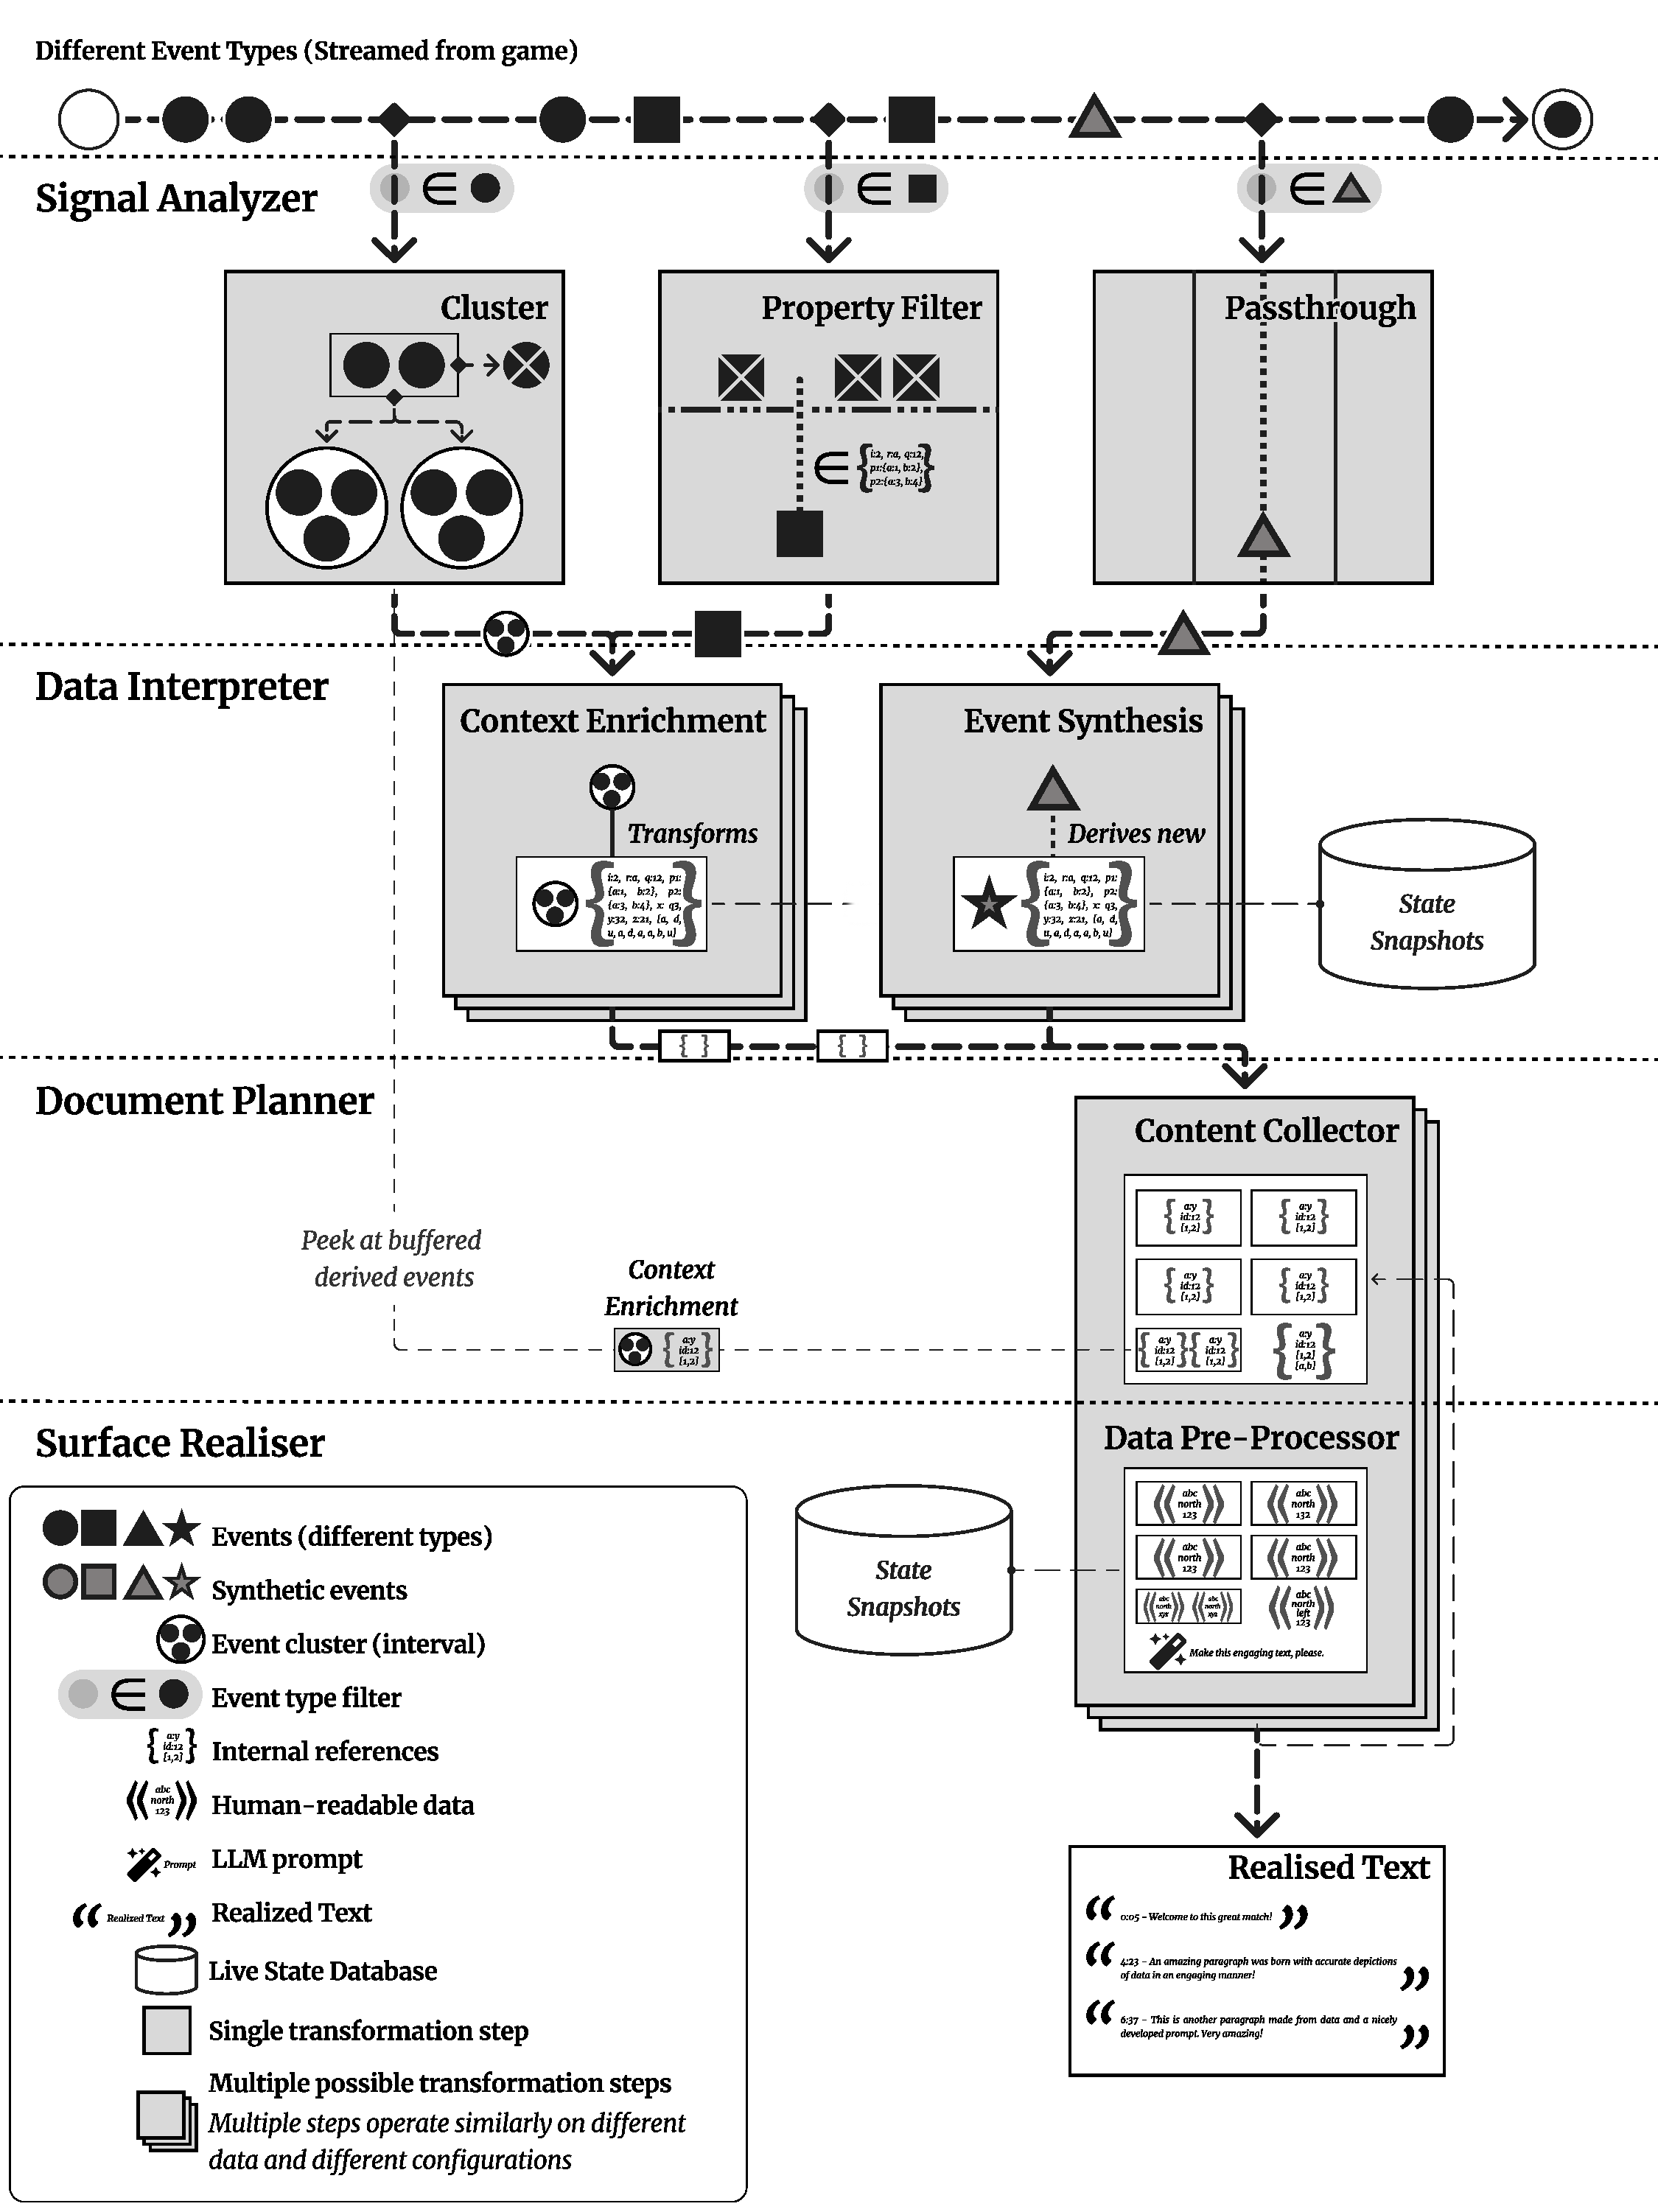
\includegraphics[width=\textwidth]{assets/data-pipeline.pdf}%
  }{%
    \fbox{\parbox{0.95\textwidth}{\centering Placeholder: missing file\\`assets/data-pipeline.pdf`}}%
  }
  \caption{Generalized overview of the \textit{SAGE} pipeline implementation, showing data flows between stages and steps. Each stage contains multiple steps; steps can have different configurations depending on the architectural module setup.}
  \label{fig:data-pipeline}

\end{figure}

The full code as well as a large dataset of CaptureAge games and generated summaries are available online \footnote{See Appendix~\ref{app:corpus} and Appendix~\ref{app:source-code} for corpus and source-code links}.

\subsection{Data Ingestion}
As a first step, we ingest the exported data from the CaptureAge API. We read the description file and load all files accordingly. The data is stored in a structure that allows for efficient retrieval of snapshot data based on time (windowId) using Arquero \cite{arquero}. It also allows for pre-filtering (e.g., to exclude thousands of entries for trees, arrows, and doppelganger entities to reduce query time) and caching for performance. We use the same structure as described in Appendix~\ref{appendix:data-schema}. In practice, we use relational queries to retrieve an initial data set and then do final filtering and processing in TypeScript. Relational queries are more efficient for large data sets, while TypeScript allows for more complex logic. An overview of what is exported from this stage can be found in Appendix~\ref{sec:example-ingestion}.

\subsection{Signal Analysis}
To mimic SAGE's online operation (processing event data incrementally as it arrives rather than from a complete batch), while using the exported dataset, we stream event data in chronological order, simulating real-time arrival. We intertwine this with a time event (Minute-Tick) every in-game minute as a heartbeat that may trigger specific time-based updates (e.g., introduction generation, or trigger a Planner flush), which also ensures that time-based buffers can be closed even when the event stream is otherwise quiet.

Signal Analysis is implemented as an event-type-specific inner pipeline: each step may emit zero or more derived events into the Signal Analysis output stream. Step configurations are defined by the architectural module setup; in our configurations, modules do not operate on overlapping event types, avoiding duplicate realization. Signal Analysis comprises two categories of steps:

\begin{itemize}
  \item \textbf{Spatiotemporal clustering:} Applied to events possessing both spatial and temporal attributes (e.g., damage events). This step groups events based on proximity in space and time, enabling identification of meaningful clusters such as fights or raids.
  \item \textbf{Property filtering:} Selects and passes only specific instants relevant to downstream processing (e.g., filtering for Castles and Town Centers among building events).
\end{itemize}

In practice, all modules use the same configuration for this stage: damage and death event clustering, building-type filtering, and passthrough for time ticks.

\subsubsection{Spatiotemporal Clustering}
Based on a comparison of spatiotemporal data clustering methods, we use a spatiotemporal variant of DBSCAN (ST-DBSCAN)\cite{shi2019, ansari2020} to cluster damage and kill events into fights based on temporal proximity and spatial location. This clustering step is the concrete implementation of the event abstraction layer, transforming the raw Instant damage events into Interval battle events. This method meets all requirements:

\begin{itemize}
  \item \textbf{Online (live) capability} - continuous clustering and ability to release clusters before processing the whole stream.
  \item \textbf{Arbitrary cluster count} - many battles can happen in parallel, and we don't want to assume a fixed number of clusters.
  \item \textbf{Arbitrary cluster shape} - we don't want to assume that battles are always spatially compact or temporally contiguous, as players may engage in hit-and-run tactics or spread out over time and space.
  \item \textbf{Arbitrary number of events per cluster} - we don't know how many events will be in a fight, and we want to capture both small skirmishes and large battles.
\end{itemize}

Input data is expected to be chronologically ordered. DBSCAN clusters data points if they are within range of at least a minimum number of other points (\texttt{minPts}) within a given radius (\texttt{eps}). This allows for two clusters to be merged if points of both are within range. This clustering allows us to identify sustained battles between players, which are critical for generating meaningful summaries.

A practical observation is that the temporal window combined with ordered input data allows for releasing clusters before the whole data stream has been processed, supporting the online capability requirement. In addition, we allow for peeking ongoing clusters and requesting them to be closed early if needed when downstream stages (Document Planner) require a summary of the current fight.

Figure~\ref{fig:online-temporal-spatial-clustering} provides an intuition for this online behavior: events arrive in chronological order, clusters can gain new events as they arrive, and clusters can be closed once no new events arrive within $\tau$ seconds.

\begin{figure}[htbp]
  \centering
  \IfFileExists{assets/online-temporal-spatial-clustering.pdf}{%
    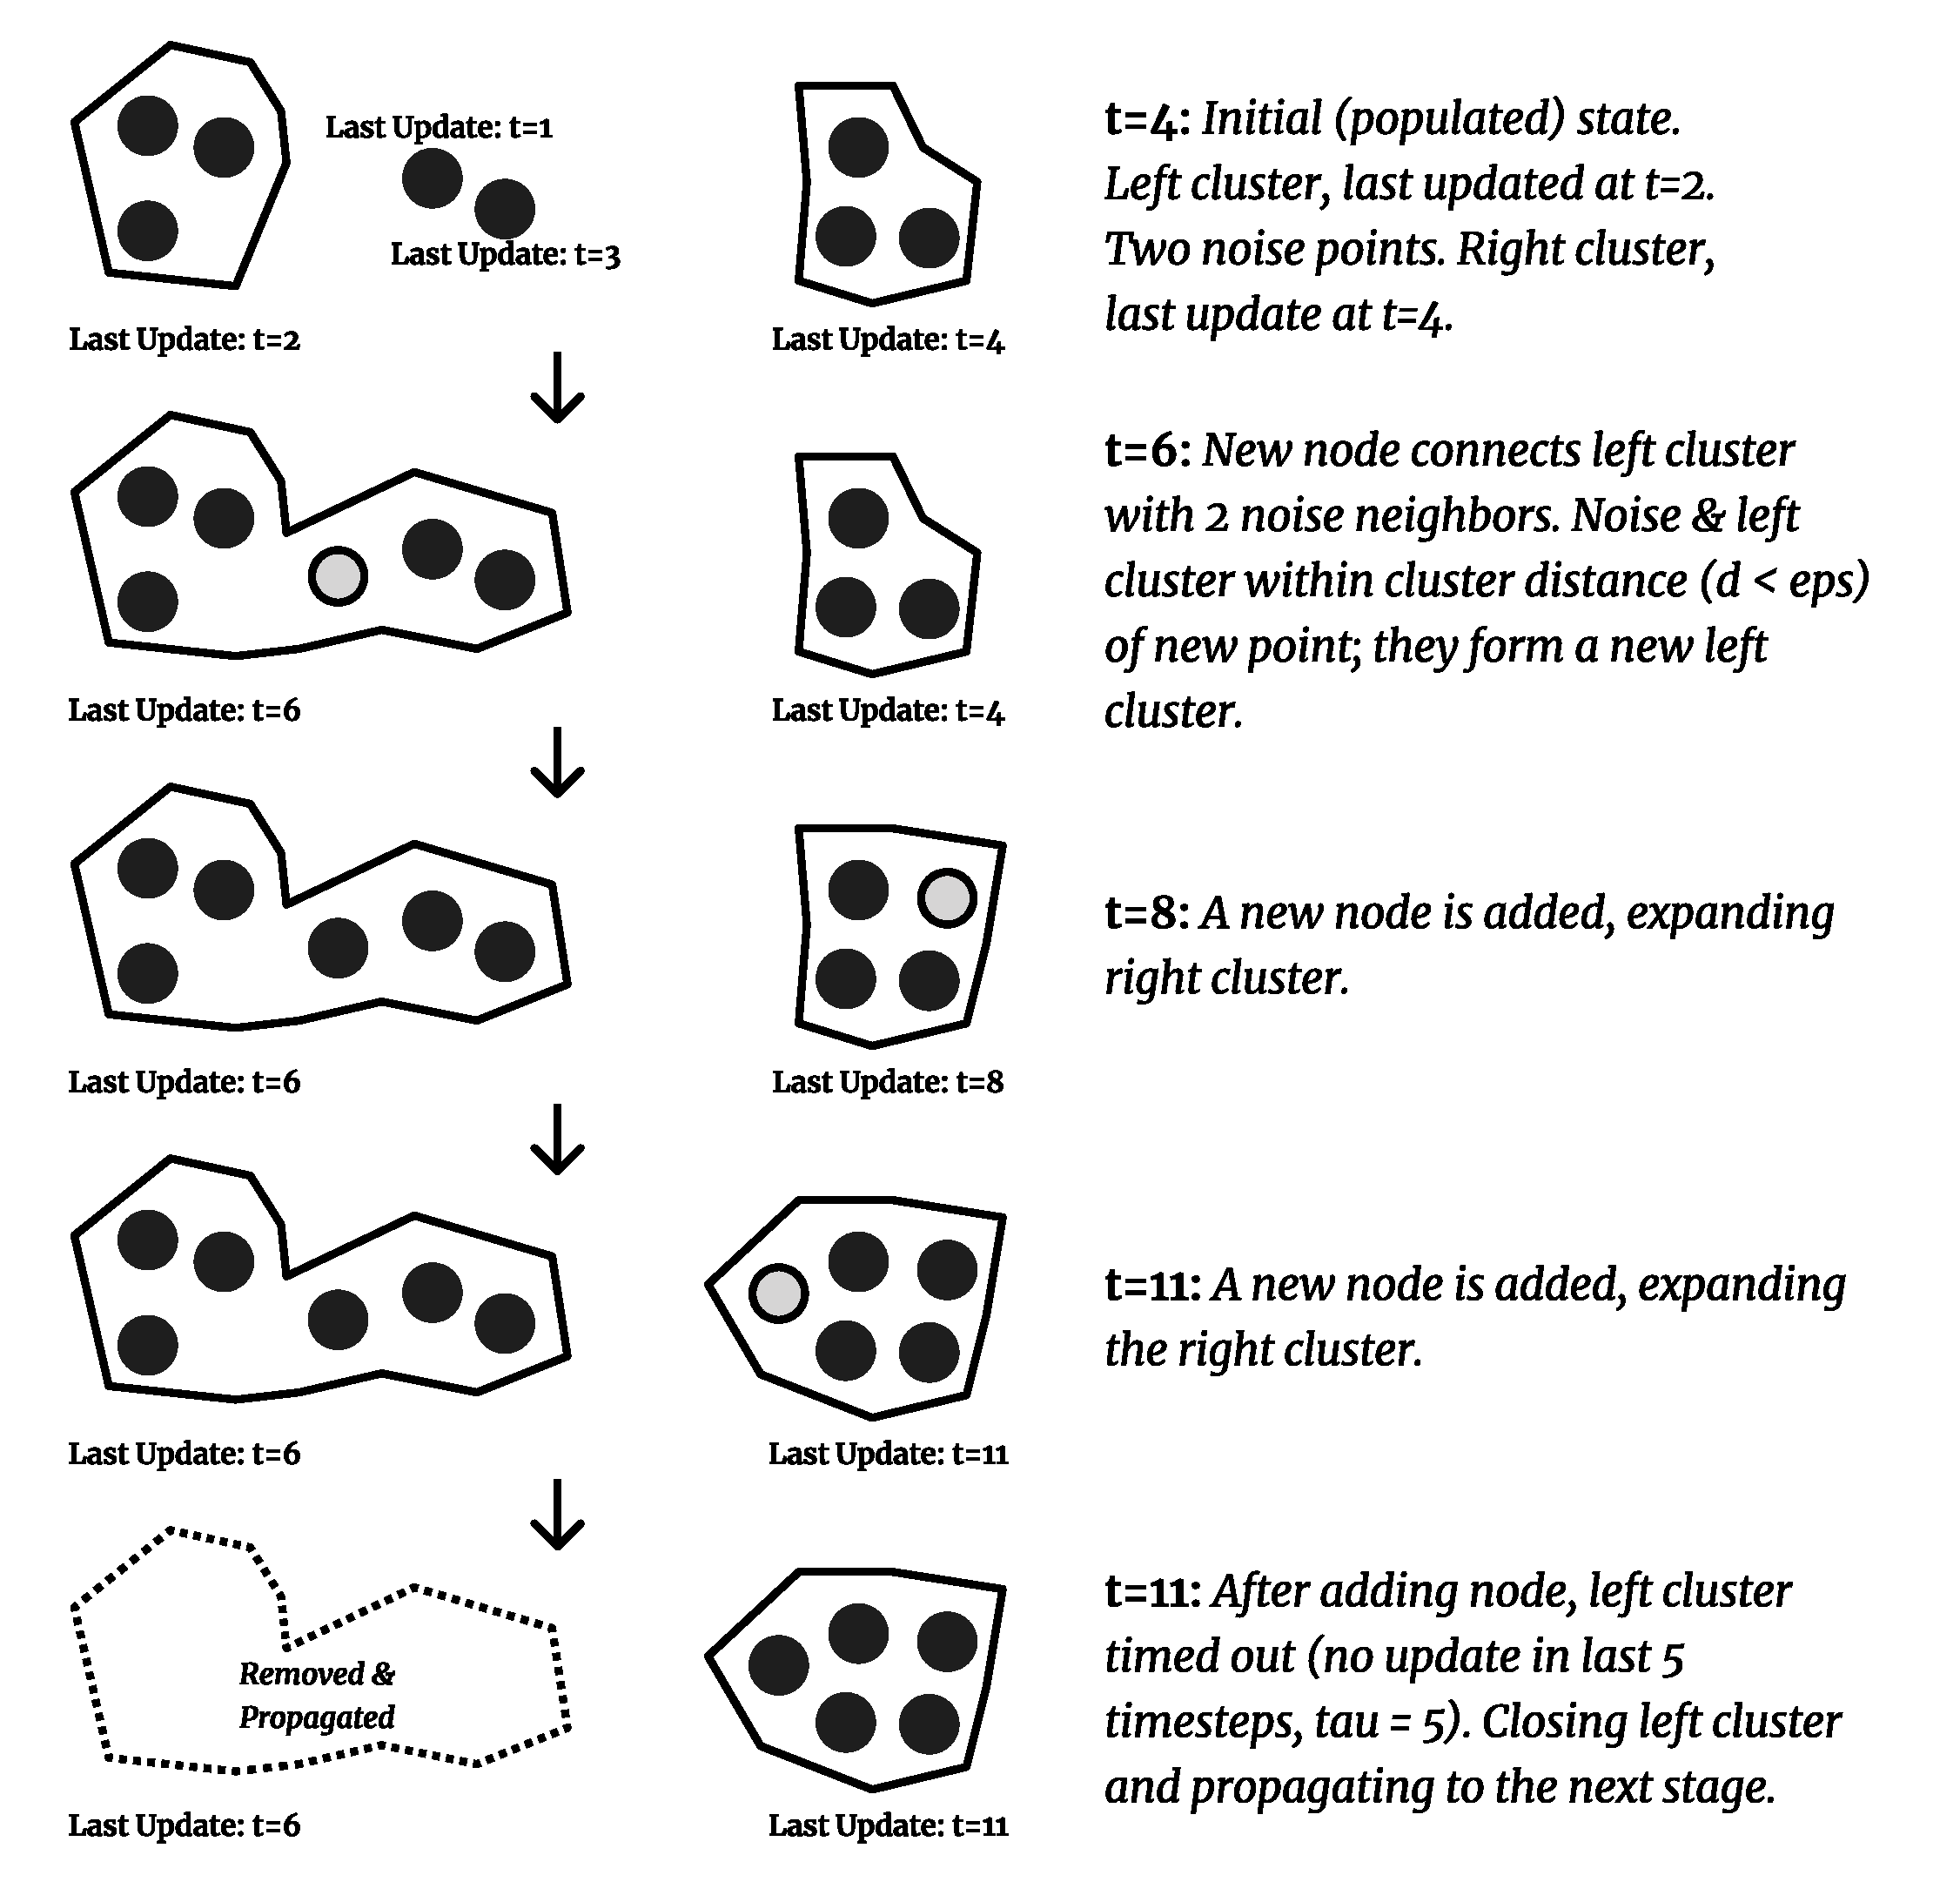
\includegraphics[width=\textwidth]{assets/online-temporal-spatial-clustering.pdf}%
  }{%
    \fbox{\parbox{0.95\textwidth}{\centering Placeholder: missing file\\`assets/online-temporal-spatial-clustering.pdf`}}%
  }
  \caption{Online temporal-spatial clustering example, showing how incoming events connect noise (t=5 through t=6), how existing clusters can gain new events (t=8 through t=11) and finally how old clusters are closed off (t=11, final). The grey circle indicates a newly arrived event.}
  \label{fig:online-temporal-spatial-clustering}
\end{figure}

Full pseudocode, implementation notes, and parameter values are provided in Appendix~\ref{appendix:signal-analysis-details}.

\subsubsection{Property Filtering}
We filter building construction events to include only narratively salient building types (Castles and Kreposts --- a "Slavs" alternative option to a Castle --- Town Centers, and Towers) to reduce noise and downstream processing load. This is implemented as a set of simple rule-based checks for entity type against a predefined list of building type IDs. While it may be interesting to explore linked construction processes (Building foundation placed, Construction started, Building completed), we leave this for future work.

\subsubsection{Minute-Tick Events}
Minute-Ticks are Synthetic Events added every in-game minute to serve as a heartbeat for periodic downstream updates (e.g., generating Introductions or flushing the Planner) and to ensure that time-based windows (e.g., temporal clustering timeouts) can still be evaluated during lulls. They are passed through to the next stage without modification; an overview of what is exported from this stage can be found in Appendix~\ref{sec:example-signal}.

\subsection{Data Interpretation}
Like Signal Analysis, Data Interpretation is implemented as an event-type-specific inner pipeline; each step can emit zero or more enriched events. This stage enriches derived (clustered) events with snapshot-based context such as location (e.g., relative to player bases), unit types, and owner data.
\subsubsection{Enrichment Steps}
We apply the following enrichment steps to each event, depending on the event type, largely aligned with the A-E-P+S framework and identified event cues from the domain analysis:

\begin{itemize}
  \item \textbf{Battles:}
    \begin{itemize}
      \item \textbf{Participants:} We identify the units involved in the battle, including their types and counts.
      \item \textbf{Casualties:} We track the units lost during the battle for each player.
      \item \textbf{Survivors:} We list the units remaining after the battle.
      \item \textbf{Army Composition:} We describe the overall composition of the armies involved (e.g., "mostly archers"). We also indicate the proportion of each unit type being in forward position.
      \item \textbf{Positional Context:} We add the named location of the battle (e.g., ``near red's forward gold'').
      \item \textbf{Economy State:} We include the current resource distribution and Villager counts.
      \item \textbf{Technology State:} We list relevant technologies researched or in progress.
    \end{itemize}
  \item \textbf{Construction:}
    \begin{itemize}
      \item \textbf{Forwardedness:} We identify for construction events whether the building is forward (closer to enemy base) or defensive (closer to own base), as this greatly influences the narrative importance of the event.
      \item \textbf{Positional Context:} We add the named location of the building (e.g., ``near red's forward gold'').
    \end{itemize}
\end{itemize}

\subsubsection{Event Categorization}
After context enrichment we categorize events into subtypes using a rule-based approach. For example, battles can be categorized into raids, full-scale battles, skirmishes, etc. based on the participants and casualties involved. This helps the Document Planner decide how to prioritize and structure the content (e.g., as \texttt{fightType} on battle events).

\subsubsection{Synthetic Events}
Based on Minute-Ticks we can also generate Synthetic Events that are not triggered by an instant-driven cue: introduction events at the start of the game, end-of-game detection, and (optionally) strategy detections (e.g., Drush --- an early Dark Age rush using Militia units --- or Scout Rush) based on the current units and buildings.

We don't add state info to construction events, since they don't typically influence the key game state metrics as much as battles do.

This stage corresponds to the Environment and Performance enrichment layers of the A-E-P+S framework. Specifically, we enrich events with Environmental information (civilization name, economy distribution, army composition, and positional context) and Performance metrics (technology states, military strength, and economic comparisons). Sensor-level data (visibility information capturing what each player can currently see through the Fog of War) is omitted for this study to reduce scope and file size, and the processing time that including per-player visibility snapshots would incur, with minimal situational impact.

For each event we can only access snapshot data for the current time tick, unless it was explicitly cached earlier, ensuring the online nature of the system. This means that enrichment must be computed incrementally and cannot rely on future game states.

A special case uses the first time-tick events to trigger introduction generation, based on the initial snapshot of the map and players.

\subsubsection{Map Positions}
To support comprehension in a text-only medium, we add stable named locations as macro-context anchors (e.g., ``red's forward gold''). This matches the finding from the user study (Chapter~\ref{chap:viewer-study}) that readers want map-position cues to connect isolated events to a coherent match state.
To report on map positions across events we query entity and terrain features using a classic spatial-only DBSCAN clustering algorithm at the start of the match. Based on the rules of Arabia (generally regarded as the most standard map for competitive play), which has standardized and consistent resources sizes and placements, we can reliably infer the location on the randomly generated map. We identify key map features such as Gold Mines, Woodlines and Sheep, as well as hills and ponds. We then give each of these a positional description relative to each player's starting location. We use three metrics for this: relative cardinal direction (N, NE, E, SE, etc.), distance (close, medium, far; crisp thresholds defined per resource), and forwardedness (a common way to describe the quality of a resource --- relative to the location of both players, implying how exposed it is to enemy attacks, we calculate an angle using a dot-product). Then we give these a name using a TypeScript port of the classic rule-based SimpleNLG Java library\cite{simpleNLG}. Compounding distance, direction, and forwardedness gives us descriptions such as ``Blue's forward, main stone mine''. We did this to obtain consistent naming between realizations, instead of relying on the LLM to generate these descriptions each time based on symbolic descriptions and coordinates. These are later used to anchor events spatially in the realization (``north-west'', or more descriptively ``neutral, north-east hill''.) While specifics are based on the Arabia map ruleset, the same approach can be applied to other maps with different resource placements and types.

We don't update the map layout as the game progresses, which is likely to happen (e.g. Gold Mines depleting or new forward expansions becoming the relevant anchor). Instead we focus on the starting state as a proof of concept. This may reduce the accuracy of later event descriptions as named anchors become stale, but generally the starting state is sufficient to ground most events.

\subsubsection{Map Introduction}
To synthesize the Map Introduction event we provide each player's name, cardinal starting location on the map and civilization. When the \textit{Expert Insights} module is enabled (see Section~\ref{sec:modules}), this introduction is further enriched with detailed civilization attributes and player playstyle information. This grounds the introduction in both the current game state and broader context: the players' identities and their civilizations' capabilities. An overview of what is exported from this stage can be found in Appendix~\ref{sec:example-interpretation}.

\subsection{Document Planning}
Document Planning receives enriched events from Data Interpretation and organizes them into content units for realization. The Planner uses event type, timeouts, and cooldown counters to (a) emit two introductions (Match Intro and Map Quality) immediately and (b) maintain a buffer of pending events. Battle and construction events are held until a periodic tick check meets one of three flush conditions: there are pending battles and their cooldown has expired, a 3-minute timeout has elapsed since the last flush, or an end-of-game event is present in the buffer.
To support live operation, the Planner can also peek at ongoing clusters in Signal Analysis when it needs a partial summary. Peeked events are explicitly marked as ongoing in the data passed to the Realizer to avoid reader confusion.

For the base module everything is passed on as it arrives, with no buffering, with the only ``event structuring'' activating for the final event to ensure that all ongoing battles are realized as well in the concluding section.

When the \textit{Event Structuring} module is active, the Planner employs a buffering strategy to identify and group related events before realization. This allows for the construction of composite events that capture parallel actions, rather than treating each event in isolation. Algorithm~\ref{alg:doc-planning} shows the core buffering and flush logic.

While Document Planning in its classical implementation is responsible for most content selection, here we forward part of this responsibility to the LLM-based Realizer. This gives the LLM more freedom to express the content in an engaging manner while still ensuring that the important content is included in the summary. An overview of what is exported from this stage can be found in Appendix~\ref{sec:example-planning}.

\subsection{Realization}
We use Gemini 2.5 Flash as the LLM-based Realizer for our system, via the Google Cloud API. The Realizer is called once per content unit generated by the Planner and returns a realized text segment.

We chose Gemini 2.5 Flash due to its low time-to-first-token latency, high throughput and large context window, in addition to high performance in ranking tasks \cite{gemini2025}. We used the June 2025 update. We configured the model with a fixed seed of 1 and a temperature of 1 for all realization calls; thinking mode was disabled. This matches the provider default temperature, and in our iterative testing it provided a workable balance between accurate reporting and engaging content. Since we were Realizing based on a predefined dataset (not live streaming data), we added additional timeouts between calls to avoid rate-limiting issues when realizing a large number of inputs in sequence.

The output of each realization call is sent back to the Document Planner to provide continuity in subsequent calls; realized segments are then concatenated to form the final summary.

\subsubsection{Context Design}
Each realization call uses a fixed system instruction that defines the model's role and constraints, plus call-specific user input. The system instruction always consists of the same parts:

\begin{itemize}
  \item \textbf{Base instruction:} Describes the LLM's role and constraints, including a specification of the input data format.
  \item \textbf{Output format:} No formatting of any kind (including Markdown and HTML) is permitted, to avoid markup artifacts and keep the output easy to present in plain-text interfaces
  \item \textbf{Output length:} Configurable word-count limit, allowing for under-generation.
  \item \textbf{Output language:} Always English.
\end{itemize}

Each content-unit type (Match Introduction, Map Introduction, Battle Events, Construction Event, Strategy Detection (Expert Insights)) from the Document Planner has a prompt associated with it with the following structure:
\begin{itemize}
  \item \textbf{Communicative goal:} Specifies what the text should express to the reader. This varies by realization type (e.g., introduction, event), but is consistent between each module.
  \item \textbf{Writing style:} Description of the desired writing style, we set the same always-enable architectural module for Writing Style here.
  \item \textbf{Additional notes:} Any further instructions for the LLM, including architectural model-specific guidance and explanations of any added data. If data is provided for this request, a prompt explains what is contained and where to find it.
\end{itemize}

For each specific realization call we then add:
\begin{itemize}
  \item \textbf{Input data:} The data to be realized, formatted as described in the Base Instruction and sent in the \texttt{``user''} role.
  \item \textbf{All previously realized text:} Added in the \texttt{``model''} role to provide context and continuity for the LLM.
\end{itemize}

Formatting influences model behavior; we provide realization inputs as JavaScript Object Notation (JSON) \cite{he2024}, which produced relatively factually correct output in our validation samples \cite{gemini2025}. We also preprocess the input data (next section) to reduce ambiguity and prompt size.

Providing previously realized text improves coherence and referential consistency, but consumes context-window budget for long matches. In practice, we found that using a large part of the context had a severely negative impact on the system's ability to use the provided factual data and to consistently follow instructions. While we originally planned to add few-shot examples, they led to worse performance in our iterative testing, and greatly reduced creativity in using contextually enriched information. Rather than balancing this with temperature, we focused on improving the other parts of the prompt, including small prompt-formatting cues to emphasize key constraints.The exact prompts (including all modules) can be found in Appendix~\ref{appendix:prompts}.

\subsubsection{Data Preprocessing}
We preprocess the data before realization to improve the LLM-based Realizer's understanding of the data and reduce mistakes. This appears \footnote{Validating this would be interesting, but is out of scope for this project.} to have two main benefits: the model is better at understanding human-readable names than numeric IDs, and compact representations reduce the tokens needed to express the same information.

Concretely, we replace opaque numeric identifiers with human-readable names (player, unit, and technology names, as well as named locations rather than \texttt{(x, y)} coordinates). For example, locations are expressed as named places (e.g., ``LoomRush's forward, tertiary Gold Mine''), which seemed to improve the model's understanding of spatial relationships in our iterative testing. While these steps could be done inside the Realizer, we apply them earlier to simplify debugging and avoid expensive multi-table join queries.

To reduce size and complexity, we also flatten repeated structures into count maps (e.g., \texttt{"food": 2, "wood": 1}). This is applied to unit and technology reports as well as battle and environment compositions (including forward-vs-total counts where needed for context). We also convert millisecond timestamps to the in-game colon format (e.g., \texttt{2:14:12}); while \texttt{1:03} is ambiguous, alternatives like \texttt{1h23m23s} reduced clarity for AoE2 readers, so we kept the colon format.

Values that can be represented as integers are not changed (e.g., \texttt{totalEcoUnits: 12}). We also updated some keys to better express their meaning (e.g., \texttt{player} to \texttt{ownerName}) for constructed buildings. An overview of what is exported from this stage can be found in Appendix~\ref{sec:example-preprocessing}.

\subsection{End-to-End Example}
To illustrate how data transforms through the pipeline, we trace a single battle event from raw ingestion to final text. This is a simplified example; actual data structures may contain additional fields, see Appendix~\ref{appendix:examples} for full details.

\paragraph{1. Ingestion}
The system receives a stream of raw ``damage'' and ``death'' events.
\begin{lstlisting}[language=JavaScript, basicstyle=\ttfamily\footnotesize]
  ...
{ type: "damage", worldX: 23, worldY: 98, worldTime: 123550, subjectEntity: 101, objectEntity: 202, ... }
{ type: "death", worldX: 23, worldY: 98, worldTime: 123550, subjectEntity: 101, objectEntity: 202, ... }
\end{lstlisting}

\paragraph{2. Signal Analysis}
ST-DBSCAN clusters these instants into a single ``battle'' interval.
\begin{lstlisting}[language=JavaScript, basicstyle=\ttfamily\footnotesize]
{
    type: "battle",
    startTimeMs: 123450,
    endTimeMs: 123550,
    data: [ ... ] // Array of clustered events
}
\end{lstlisting}

\paragraph{3. Data Interpretation}
The event is enriched with context (participants, location, economy) and classified.
\begin{lstlisting}[language=JavaScript, basicstyle=\ttfamily\footnotesize]
{
    type: "battle",
    location: "Red's forward Gold",
    player1: { participants: ["Archer", ...], casualties: ["Archer", ...] },
    player2: { participants: ["Skirmisher", ...], casualties: [] },
    fightType: "skirmish",
    ...
}
\end{lstlisting}

\paragraph{4. Document Planning}
The Planner selects this event for realization and structures it into a content unit.
\begin{lstlisting}[language=JavaScript, basicstyle=\ttfamily\footnotesize]
{
    type: "multipleEvents",
    startTimeMs: 123450,
    endTimeMs: 123550,
    battles: [ ... ], // The enriched battle object(s)
    previousRealisation: [ ... ] //  supplied as "model" messages
}
\end{lstlisting}

\paragraph{5. Realization}
The LLM generates the final commentary based on the content unit and prompts.
\begin{lstlisting}[language=JavaScript, basicstyle=\ttfamily\footnotesize]
  ``A skirmish breaks out at Red's forward gold! Red's Archers are caught out by Blue's Skirmishers, taking heavy losses.''
\end{lstlisting}

For a complete list of data structures at each stage, see Appendix~\ref{appendix:examples}.

\section{Limitations}
We acknowledge several limitations in our system design:
\begin{itemize}
  \item \textbf{Data scope:} We rely on CaptureAge's reconstructed state and Instant Events; any omissions or inaccuracies there propagate downstream. We also cannot realistically iterate quickly on the amount of data that is provided by CaptureAge, since it requires re-running games and re-processing them to get old data; to cope with this, we use large snapshot windows. This also allows us to request data from earlier in the game, which is useful because our pipeline buffers data when clustering events from the stream. In a true live setting this would not be possible; instead we would need to retrieve data as we receive the stream or cache it for forward use.
  \item \textbf{Event detection:} Our Signal Analysis uses heuristic rule-based clustering; complex patterns may be missed or misclassified. In Section~\ref{sec:pipeline-implementation} we describe the clustering method we selected and discuss its limitations, aiming to reduce misclassification and omission. Furthermore, we have primarily focussed on clustering battle-related events, with some "gaps" filled with construction events, and per-module additions. This was a targeted approach, but more events can make for a richer narrative. For the purposes of this research, we accept this limitation, since we are more interested in the effect of context enrichment and event structuring on engageability.
  \item \textbf{LLM realization:} While flexible, LLMs can produce inconsistent phrasing or factual errors; we mitigate this by providing factual data but cannot eliminate it entirely. Our approach of enriching the data with E-P+S data and the \textit{Expert Insights} module aims to reduce these errors by providing more context to the LLM, essentially using Retrieval-Augmented Generation, i.e., explicitly retrieving relevant facts from the game state and feeding them into the prompt \cite{lewis2020}. In our development, we found LLMs preferable to the rule-based Realizers we initially planned to use. In addition, LLMs implicitly encode vast amounts of domain knowledge, effectively serving as a soft ontology. While useful, this does mean that we have less control over the exact linguistic output compared to a rule-based Realizer; to counteract this, we use negative prompting to avoid unwanted phrases.
\end{itemize}
Knowing these limitations helps with implementation-level decisions and with defining realistic outcomes for the development phase.

\subsection{Evaluation Constraints}
Since we want to evaluate engageability, we need to be able to test different configurations of the system. The modular design allows us to swap out modules and ablate them to test their effect on engageability. This requires testing many different configurations, which can be time-consuming. In addition, the generated text needs to be of a length that is reasonable to read for participants in a user study. Since the number of modules has a multiplicative effect on the number of configurations, we limit ourselves to varying two modules (\textit{Expert Insights} and \textit{Event Structuring}), while keeping the Writing Style module always enabled in our study conditions to ensure a baseline level of engageability. We also aim to shorten the generated text by limiting the maximum output length of each text in the Realizer, as well as removing less important events in the Document Planning stage and not reporting on lulls. This breaks with \citet{lewandowski2012}'s definition of minute-by-minute reports, where sometimes non-descriptive information is reported to fill lulls. We accept this limitation because we want to focus on engageability through descriptive information and event-driven reporting.

\section{Architectural Modules}
\label{sec:modules}

We aim to evaluate different strategies for enriching the generated text, based on our findings in the previous chapter and our aim to increase engageability. In particular, we want to test the effect of adding contextual information and how to deal with parallel events and their relations. \citet{callaway2002} propose an ablative design using architectural modules, where modules can be swapped or ablated to test different strategies for enriching the generated text. We follow a similar approach, introducing modules that can influence any stage of the pipeline by adding steps. This allows us to experiment with different enrichment strategies without altering the core pipeline.

\begin{figure}[htbp]
  \centering
  % Avoid build errors if file is missing
  \IfFileExists{assets/pipeline-modules.pdf}{%
    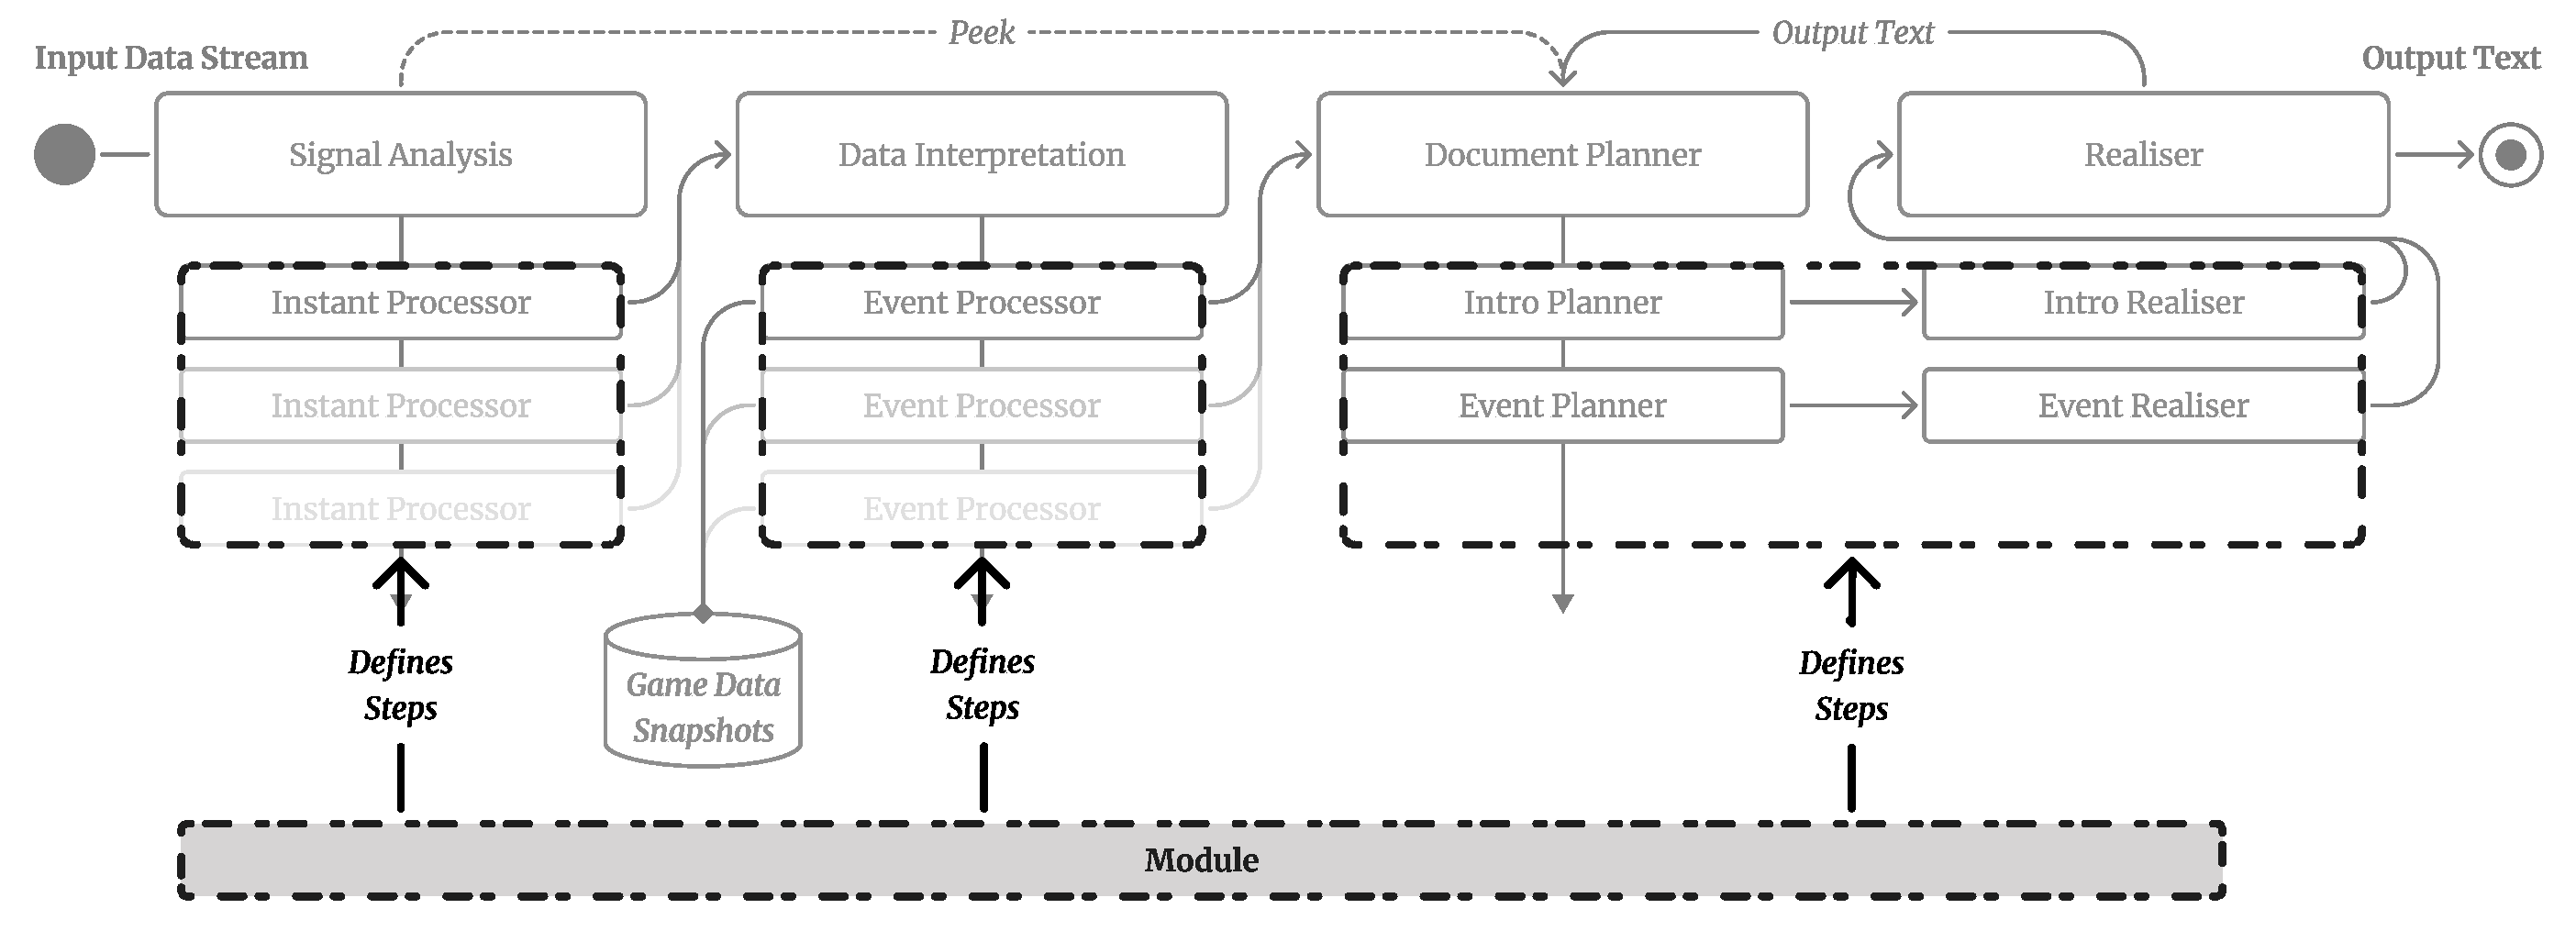
\includegraphics[width=\textwidth]{assets/pipeline-modules.pdf}%
  }{%
    \fbox{\parbox{0.95\textwidth}{\centering Placeholder: missing file\\`assets/pipeline-modules.pdf`}}%
  }
  \caption{Modules that can be independently enabled or disabled to test different strategies for enrichment of the generated text. A module can influence any stage of the pipeline by adding steps.}
  \label{fig:pipeline-modules}
\end{figure}

We test three engageability-related strategies by enabling and disabling modules independently:
\begin{enumerate}
  \item \textbf{Adding contextual information:} This is often provided by (color) commentators in live sports commentary. Although previous research has not directly validated its effect, it is frequently mentioned as an important factor \cite{li2020, margetis2023}.
  \item \textbf{Explaining parallel events:} Providing explanations for parallel events supports better understanding of the game state, as suggested by related work \cite{cheung2011starcraft} and anecdotal evidence from shoutcasters in our own analysis.
  \item \textbf{Stylistic variation:} Testing the effect of stylistic variation on engagement, as highlighted by analysis \cite{lewandowski2012, byro2017, gustin2020}, to see if mimicking the engaging style of esports shoutcasters improves reader engagement.
\end{enumerate}

We introduce three top-level architectural modules. Their inclusion is driven by experimentation goals rather than necessity for basic functionality. Each module can add steps in Signal Analysis, Data Interpretation, Document Planning, and Realization. Since modules can work together we ensure that any added step consumes data made available by upstream stages and produces outputs that remain compatible with downstream stages. In particular, Document Planning and Realization operate in pairs, so that each Planner output type has a corresponding Realizer configuration that produces a single realization for each content unit.

Figure~\ref{fig:pipeline-modules} illustrates how modules can influence any stage of the pipeline by adding steps. In our evaluation we vary \textit{Expert Insights} and \textit{Event Structuring}, while keeping the Writing Style module enabled to ensure a baseline level of engageability (see Evaluation Constraints above).

\subsection{Event Structuring}
The optional \textit{Event Structuring} module operates primarily at the Document Planning stage but influences the entire pipeline. Its main responsibility is to select the most important events, group them into coherent sequences, and provide a better trade-off between supportive context and events. This should be done in a way that supports reader understanding of complex, simultaneous actions.

\subsubsection{Document Planning}
The \textit{Event Structuring} module operates on the Planner's buffering mechanism. Instead of passing events immediately to the Realization stage, the Planner buffers events to identify temporal and spatial overlaps. Specifically, the prototype uses a buffer of at most 180 game seconds or 5 events. Within these buffers, events are sorted by importance (e.g., prioritizing large battles or those with significant economic damage over small skirmishes) to determine the narrative focus. It also ``peeks'' at the Signal Analysis stage to check for ongoing events that might be relevant to the current buffer, ensuring that related events are not split across different realization cycles.

\subsubsection{Realization}
When the \textit{Event Structuring} module is active, the Realizer receives grouped events instead of individual ones. The prompts are adjusted to instruct the LLM to weave these events into a single narrative segment (see Appendix~\ref{appendix:arch-modules-prompts}). This includes guidance on how to handle temporal overlaps and spatial relationships, ensuring that the summary reflects the complexity of simultaneous actions. With this, the Realizer is responsible for deciding both what information to include and which events to report on. We also reduced the number of updates. After experimentation, we gave it an additional 50\% word budget to still aim for the same document length range (500--800 words). Since the Document Planner decides how to group events, the Realizer can be consistent with the word budget per content-unit, to help focus on the most important events.

Following our previous observations, we prompted the LLM to emphasize Information Asymmetry for increased engagement. It was also told to clearly indicate when multiple events are happening at the same time using temporal Cues in the longer paragraphs, and the use of ``Transitional'' phrases such as ``Meanwhile, on the other side'', ``But their opponent doesn't know'', or ``What are they planning?'' to help readers follow the concurrent actions.

\subsubsection{Experiment: Agentic Document Planning}
We attempted a single, simple agentic approach as well, where the LLM was given a prompt to alternatively return a keyword (``<DEFER>'') to postpone realization to gather more events. It was given the task to reduce reporting on an Age (technology) progression basis (i.e., every minute before Castle Age, every 3 minutes after Castle Age). It was given the aim to use this mechanic to keep readers engaged. However, in our tests, it only postponed realization on a few occasions, ignoring the explicit frequency instructions to do so.

\subsection{Expert Insights}
The optional Expert Insights module enriches the raw game data with domain-specific knowledge, connecting observable facts to their strategic significance. This enrichment occurs primarily during the Data Interpretation stage. There we rely on two mechanisms: newly derived Synthetic Events and context enrichment of existing events. We also provide causality information (e.g., ``against early Archer attacks, defenses need to stretch a larger area to counter their arrow's range'') in the prompts for the LLM-based Realizer to leverage this information effectively. These prompts include data descriptions and minor points to allow it to better use the data and understand the implications.
Domain Knowledge is provided in Data Interpretation, while Analytical Knowledge is provided in the Realization stage.

\begin{itemize}
  \item \textbf{Player Data:} Adds context about the players, such as their known playstyles (e.g., ``aggressive'', ``defensive'') and historical performance. This data was retrieved from a static knowledge base compiled from community resource Liquipedia~\cite{liquipedia} and the author's knowledge. It includes details such as player names, clan affiliations, and typical strategic tendencies. Since players were anonymized in our user study, we include this background primarily to support reader understanding and to test whether prior player knowledge affects ``delight'' \cite{oshimi2015}.
  \item \textbf{Civilization Data:} Injects information about the civilizations played, including their unique strengths, weaknesses, and key units. This information, sourced from the Age of Empires II Fandom Wiki~\cite{aoe2wiki}, helps to explain \textit{why} certain events might be happening (e.g., a civilization's economic bonus enabling a faster advance). This injection is done for all battle events, since civilization traits often influence combat outcomes.
  \item \textbf{Strategy Detection:} Uses a fuzzy logic filter to detect high-level strategies (e.g., ``Tower Rush'', ``Fast Castle'') based on the distribution of units, buildings, and technologies. This allows the system to label a collection of events with a strategic intent. The Data Interpretation stage emits detected strategies as derived Synthetic Events, on a per Minute-Tick basis.
\end{itemize}

\subsubsection{Fuzzy Strategy Detection}
The strategy detection mechanism is implemented using a simple fuzzy logic engine that evaluates the game state against a set of predefined strategy templates. This approach allows for the detection of strategies that are not strictly binary but rather exist on an interval of confidence. In essence: ``If you see 2 archers we are likely seeing an archer rush, but if you see 5 archers we are certain''. These statements can be chained and combined: ``However, this strategy usually only occurs before 12 minutes and never after 15 minutes.'' There are many strategies in Age of Empires II, each with its own set of indicators which are also used by human commentators and players to identify them. Fuzzy sets are a methodology to combine these indicators into a single confidence score.

This system may deserve a full section, but it only contributes as a small part of an architectural module, so we provide a concise overview here; an example configuration is provided in Appendix~\ref{appendix:fuzzy-logic}.

\paragraph{Evaluation Input Fields}
Each strategy template defines a set of criteria based on the following input fields:
\begin{itemize}
  \item \textbf{Unit Criteria:} Evaluates the count and position of specific unit types. For example, a ``Tower Rush'' strategy might require a high number of Villagers in a forward position.
  \item \textbf{Building Criteria:} Similar to unit criteria, but for buildings. It checks for the presence, count, and position (forward vs. defensive) of key structures.
  \item \textbf{Technology Criteria:} Checks the state of specific technologies (researched, researching, or queued). This matters for timing-based strategies like ``Fast Castle''.
  \item \textbf{Villager Distribution:} Analyzes the economic focus of a player by evaluating the number of Villagers gathering specific resources (e.g., high stone allocation for a Tower Rush).
  \item \textbf{Constraints:} Hard constraints such as the current Age or Civilization, which act as binary filters.
\end{itemize}

\paragraph{Scoring and Combination}
Each criterion is evaluated using trapezoidal fuzzy sets, which map a numerical input (e.g., unit count) to a membership value between 0 and 1. Typically, these sets allow for a linear transition of confidence. For example, if we see 3 Militia, we might be 100\% confident that the ``Enough Militia Present'' criterion is met for ``Drush'' strategy, while 0 Militia gives 0\% confidence, and 1-2 Militia yields a value between 0-100\%.

However, we also employ these sets to enforce crisp requirements. By defining a trapezoid with a vertical ``cliff'' (e.g., using the \texttt{atLeast(n)} helper), we can create hard constraints where any value below $n$ has 0 membership and $n$ or above has 1. This allows the fuzzy logic system to handle binary conditions (like ``Must have Loom researched'' or ``Must have at least 2 Villagers on Stone'') alongside graded ones.

These individual membership values are then combined to form an overall confidence score for the strategy.

\begin{itemize}
  \item \textbf{Input Field Evaluation:} Each input field uses fuzzy sets defined by parameters like `atLeast`, `atMost`, or `between` to determine how well the current state matches the expected value.
  \item \textbf{Combination Logic:} Individual field scores are combined using standard fuzzy logic operators. Typically, criteria within a category are combined using a fuzzy AND (the minimum of all scores is propagated), while different categories can be weighted or combined to form the final score.
\end{itemize}

\paragraph{Runtime Execution}
In practice, the system iterates over all defined strategy templates for each Minute-Tick event.
\begin{enumerate}
  \item \textbf{Time Window Check:} First, the system checks if the current game time falls within the valid time window for the strategy (e.g., a ``Dark Age Rush'' is only valid in the early game).
  \item \textbf{State Evaluation:} If the time window is valid, the engine evaluates the current game state against the template's criteria to compute a confidence score.
  \item \textbf{Thresholding \& Selection:} Strategies with a confidence score below a minimum threshold (set to 0.3) are discarded. Among the remaining candidates, the strategy with the highest confidence score is selected and emitted as a Synthetic Event to the Data Interpretation stage.
\end{enumerate}

\paragraph{Strategy Template Generation}
The templates were created by an LLM (Gemini 2.5 Pro, version June 2025 (VSCode Copilot)), based on a list of strategies to detect and an overview of each leverage point (units, buildings, technologies, villager distribution). No additional information was given to the LLM about how these strategies manifest in-game, relying on the LLM's knowledge to create the initial templates. These were then manually reviewed and adjusted to ensure correctness and feasibility.

This is an interesting finding in itself, as it shows that LLMs can be used to generate domain-specific knowledge representations that can then be operationalized in a (much more computationally efficient, accessible and explainable) rule-based system, without prior training.

\subsubsection{Data Interpretation}
Based on the event type, the Expert Insights module enriches events with additional data: Match Introduction events are enriched with player and civilization data, Battle events are enriched with civilization data, and Synthetic Strategy Events are emitted as detected.

\subsubsection{Document Planning}
The \textit{Expert Insights} module modifies the Document Planner for strategy reporting. When a strategy is detected, it's always prioritized, ensuring that it's realized as soon as possible. The detected strategy is included in the context for all subsequent realizations, allowing the LLM to reference it when describing events. For this the Document Planner memorizes the last detected strategy for each player, and the time it was detected.

\subsubsection{Realization}
Each Realizer is told exactly where to find the additional \textit{Expert Insights} data and how it is structured. We provide instructions on how to interpret the data given several Analytical Knowledge examples (see Appendix~\ref{appendix:arch-modules-prompts}). This includes explanations of civilization strengths and weaknesses. For example if Gold is forward and your opponent is likely to make Archers (e.g., the Britons civilization), then wider walls or even a tower may be advisable. We include a small number of high level examples, explicitly pre-conditions and the possible implications, to help the LLM understand how to combine these data points effectively.

\paragraph{Negative Prompt}
Despite a general prompt asking the LLM to ground all its output in provided information and facts, it would still attempt to provide expert knowledge. To combat this, we explicitly added a negative prompt as a Realization-only module. This reduces the risk that, when no \textit{Expert Insights} data was provided, the LLM would hallucinate such information (or, in some cases, correctly infer it). This was tailored to each event type (e.g., for the Match Introduction it was given: ``Report only facts from the provided data - avoid general game knowledge.'').

\subsection{Writing Style}
The Style module is a stylistic configuration that operates at the Realization stage. Unlike the other modules, it does not alter the data flow or structure but adds a small prompt influencing how content is expressed.

We based this on the findings by \citet{lewandowski2012} on how to shape our target register of live text commentary (or online sports commentary, OSC). In particular the simple present use, copula be deletion, and use of spatial and temporal anchoring.

Initially we also requested the use of metaphorical language \cite{byro2017, gustin2020}, but the LLM was not able to apply this in a way that the author felt was in line with community expectations, so we removed this aspect. Instead we used simpler language to prompt engaging language.

\subsubsection{Realization Stage}
The Writing Style module only had a Realization-stage-specific influence, adding a simple prompt (detailed in Appendix~\ref{appendix:prompts}):
``Use dynamic, exciting language sparingly to maintain engagement while keeping content concise. Most content should be written in the simple present tense, feel free to use copula be deletion where appropriate.'' as the Writing Style component of the prompt.

This directly reflects the main findings, while encouraging the LLM to balance engagement with factual reporting.

An example sentence generated with this module active is:
\begin{quote}
  \textit{37:24 - A brutal major battle near red's Town Center! Blue's army is decimated, losing 27 units, while red loses only 14, mostly Villagers. Red still holds a strong military advantage!}
\end{quote}

This clearly shows copula be deletion (``\underline{There is} a brutal major battle...''), with most of the sentences written in the simple present tense, as well as the use of dynamic adjectives (``brutal'', ``decimated'') to increase engagement.

We procedurally added the timestamp to improve consistency across realizations, which the LLM struggled with. In general, it was able to add the positional data (near red's Town Center). \footnote{It's interesting that it was this good at supplying positional data, compared to adding consistent timestamps. This may be due to the fact that positional data is more semantically relevant to the event, while timestamps are more of a meta-data aspect, thus not being prioritized by the LLM.}

\section{Conclusion}\label{sec:system-design-conclusion}
The prototype delivers a modular, incremental pipeline that meets our feasibility goals: factual summaries based on high-fidelity game data, a clear structure aligned with our narrative design focusing on engageability, and extensibility through architectural modules.

\subsection{Discussion}
During prototype development, we adhered to five main criteria to ensure progress toward a functional system, and evaluated these criteria iteratively on a single representative match based on the author's judgment and checking the completeness at key points in the match (e.g., after the first big battle, after the first Castle Age, etc.):
\begin{itemize}
  \item \textbf{Structural Completeness:} Structural completeness was realized through deterministic Document Planning, ensuring that all key narrative components (introductions, battles, constructions) were represented in the final summary.
  \item \textbf{Data Correctness:} This is the most critical criterion, as the system's credibility hinges on accurate reporting, while rule-based event detection is limited in its accuracy. We validated correctness through manual review of generated summaries against the original game data and video-based shoutcasts, aiming to confirm that reported events and statistics matched in-game occurrences. It's not feasible to do this for every summary generated during iteration. However, the final evaluation did not reveal surface-level issues, and a preliminary run of four additional games (used for the evaluation in Chapter~\ref{chap:eval}) also did not surface obvious correctness problems.
  \item \textbf{Reporting Density:} Balancing the frequency of reported events was important. We found that the base case, realizing every event required a reduced target number of words per event to avoid overly long summaries. The \textit{Event Structuring} module helped improve this by grouping related events, allowing for richer context without overwhelming the reader, generally creating shorter summaries.
  \item \textbf{Readability:} We rarely found readability issues during iterative testing, mostly related to the LLM's output. From time to time a repeated sequence was found, which can be mitigated by tweaking the temperature, but we found this not frequent enough to warrant straying from the default recommended temperature. While we cannot say that the text is engaging without a formal evaluation, the output includes many of the stylistic elements we aimed for, such as simple present tense and copula be deletion, as well as spatial and temporal anchoring, while using dynamic language to increase engagement. It should be noted that the LLM sometimes realized text in other tenses, but this is technically permitted by the prompt, in line with prior findings \cite{lewandowski2012}. Informal feedback from other readers indicated that the summaries were easy to read and follow, with a coherent narrative flow, reducing a potential need to add a static visual modality for grounding the text.
  \item \textbf{Module Functionality:} Each architectural module was tested in isolation to confirm it contributed to the overall system. Since there is a clear interaction between \textit{Event Structuring} and the output (it increases the number of words per output section), we tested each module's interaction with \textit{Event Structuring} as well. In our tests, all modules behaved as expected.
\end{itemize}

These criteria served as effective guardrails, allowing us to iterate rapidly on a single representative match before scaling up.

However, we have not evaluated the system beyond a limited data set due to the scope of this thesis. This limitation is amplified by the non-deterministic nature of LLMs, where even small data differences can yield vastly different outcomes. A particular risk lies in the generalizability of detection steps—specifically fuzzy strategy detection (any parameter) and clustering sensitivity (\texttt{eps}, \texttt{minPts} and \texttt{tau}) — to different game scenarios and player styles. Fortunately, the modular architecture allows these components to be swapped for robust implementations in future work.

\subsection{Future Work}
Several areas for improvement emerged during development, particularly regarding the LLM's context window and data handling. We observed that some instructions in prompts, particularly stylistic and formatting directives, were ignored over time in longer matches, likely due to the prompt size (the data in particular) being large, causing context overflow. Future iterations could implement ``differential snapshots''—focusing on state changes rather than full data dumps—to reduce token usage and highlight standout changes. Agentic approaches could go further by making retrieval goal-driven: the system could decide what to retrieve for a given communicative goal (e.g., emphasize spectacle in a decisive fight, but emphasize strategic context or expert insight during lulls), and avoid enriching with facts that are not currently useful for realization. However, this shifts work into iterative retrieval and may increase response time without careful caching/prefetch strategies.

Reducing prompt size is also important for economic viability. In our current prototype configuration, realizing a full match can cost on the order of \$0.10 in API usage (driven largely by the amount of structured data passed into the Realizer), which makes full-match generation hard to justify in many real-world settings without more aggressive compression.

The current focus on start and end states of battles, while useful for visualization, can occasionally lead to repetitive narratives. Future work should explore ways to better capture the dynamic flow of combat. This can be done by passing the exact battle logs, or by implementing more sophisticated event detection that captures key turning points within battles.
Furthermore, while our early enrichment strategy is conceptually strong, it risks time misalignment due to the minute long windows, and looking up the data at Interpretation time, instead of at data ingestion time. In a live system, this means either enriching eagerly (at ingestion time) or preserving immutable snapshot views keyed to event/ingestion time, so later planning and realization cannot accidentally enriching against a ``newer'' (and therefore untruthful-for-that-moment) state. Adopting more advanced statistical methods or specialized models for state tracking—moving away from purely LLM-based enrichment—could improve practicality.

Requesting the LLM to generate a structured representation of the content before realization could also improve factual accuracy, as it would force the model to explicitly outline the information it plans to include. This intermediate step could be validated against the input data, reducing hallucinations, and would provide a clearer audit trail for the generated content.

Finally, the system's modularity opens the door for a generalized approach. By defining game-specific Signal Analysis and Data Interpretation modules, the core Realization and Planning components could be reused across different esports or even other time series data reporting domains.

The prototype is modular, incremental, and meets its feasibility goals: factual summaries from high-fidelity data, a structure aligned with the narrative design, and extensibility through architectural modules. Whether this design effectively improves engagement, and holds up in a less controlled environment is evaluated in the next chapter (Chapter~\ref{chap:eval}).